\documentclass[12pt, demo]{article}
\usepackage[margin=1in]{geometry}
\usepackage{pythontex}
\usepackage{tabularx}
\usepackage{graphicx}
\usepackage{titling}
\usepackage{amsmath}
\usepackage{ragged2e}
\usepackage{float}

\title{Using Machine Learning to Predict Typing Speed}
\author{jjr117}
\date{}

\newcommand{\code}[1]{\texttt{#1}}

\newenvironment{textexamples}
  {\medskip\par\setlength{\parindent}{0pt}}
  {\par\medskip}

\graphicspath{{assets/}}

\begin{document}

\maketitle

\section*{Introduction}

One of my hobbies is competitive typing, where I compete with my friends to type a text as quickly as possible. I often use a website called TypeRacer, where your goal is to drive a racecar to the finish line, and the position of your racecar is determined by how many words you've typed correctly in the quote:

\begin{figure}[H]
	\caption{A screenshot of a typing competition on the website \textit{TypeRacer}}
	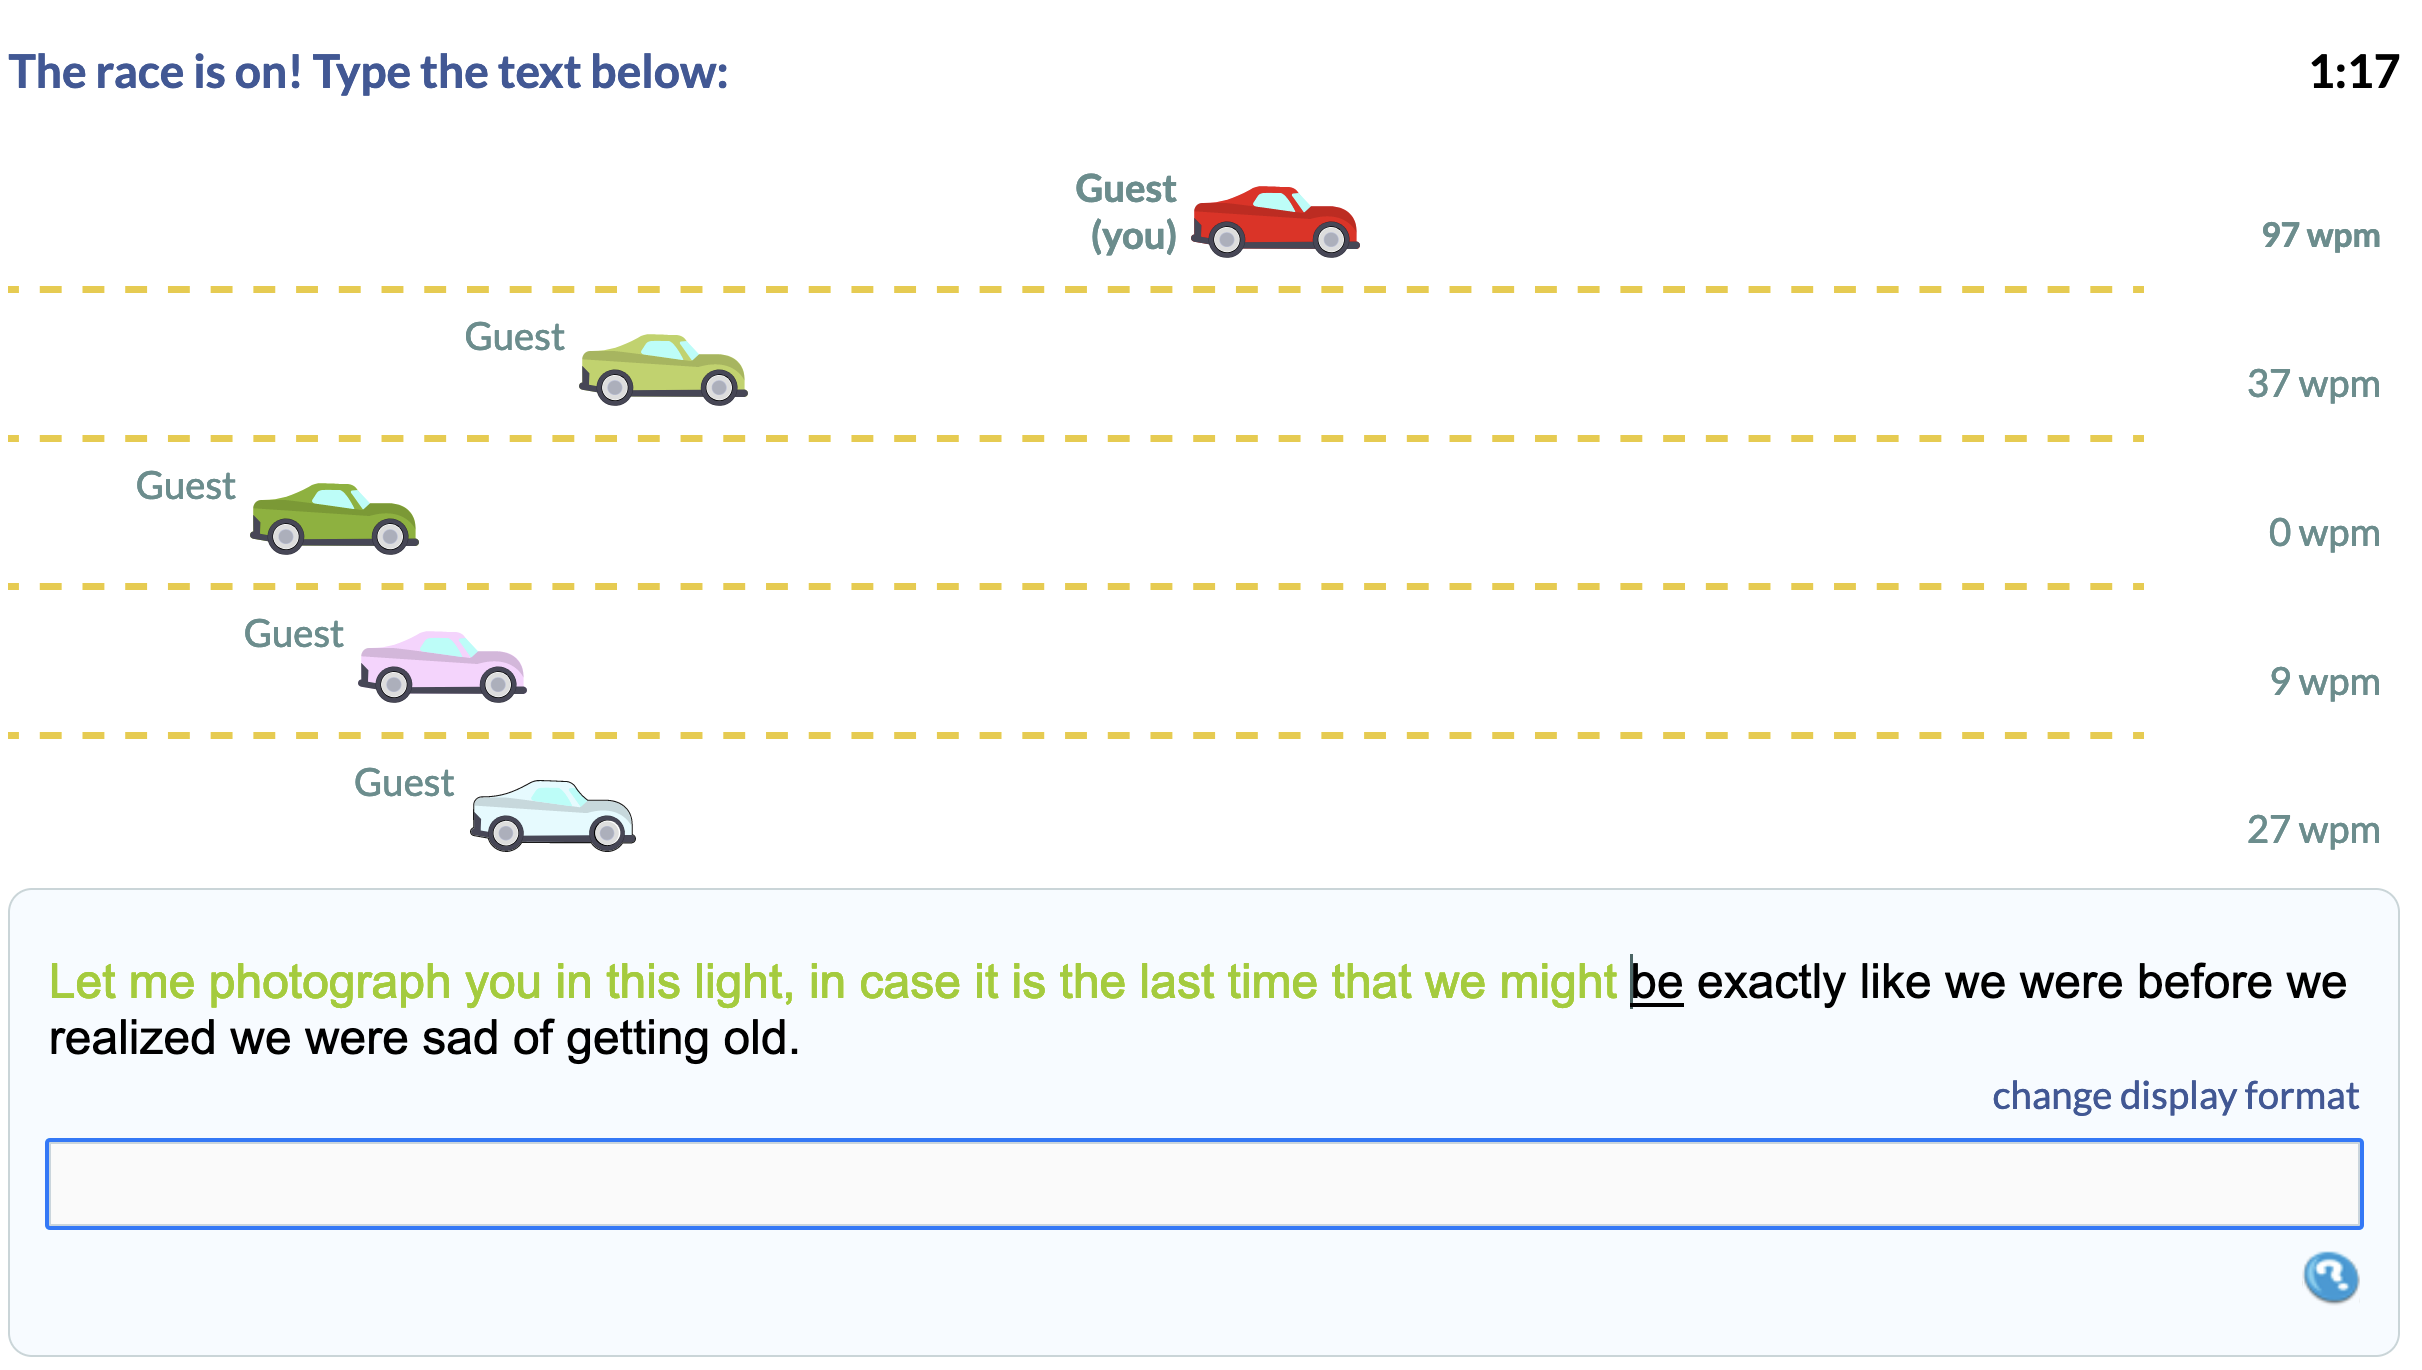
\includegraphics[width=\textwidth]{typeracer.png}
\end{figure}

Your score is a measurement of your average typing speed at the end of the race. Typing speed is measured in the units "words per minute" ("wpm" for short), and each word is defined as five characters.

In TypeRacer, your typing speed determines the types of texts you'll be presented with: a lower typing speed gives you easier texts, while a higher typing speed gives you more difficult texts:

\begin{figure}[H]
	\caption{Two different possible texts in TypeRacer. On the left, an easy text, and on the right, a more difficult text.}
	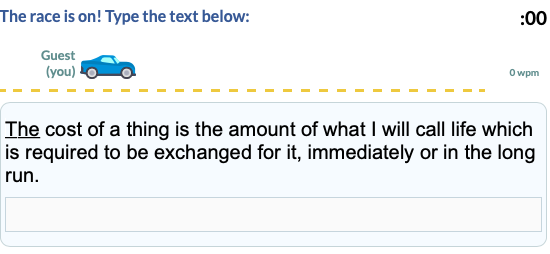
\includegraphics[width=0.5\textwidth]{easy-text.png}
	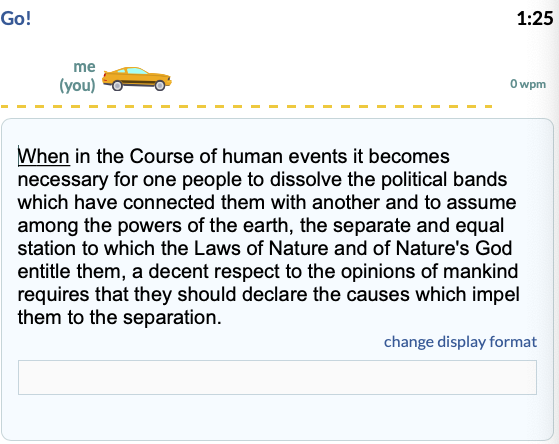
\includegraphics[width=0.5\textwidth]{hard-text.png}
\end{figure}


However, not all texts are created equal. Some texts are harder to type than others, whether it's from having longer, more complex words, frequent capital letters, numbers, etc.

Predicting the difficulty of a text is useful. For example, the typing site that I practice on, TypeRacer, will display different sets of texts depending . For example, these are two quotes that can appear in a TypeRacer race:


Even though Quote 1 is shorter than Quote 2, the difficult word at the start of Quote 1 makes it significantly more difficult to type.

Currently, the way TypeRacer classifies the difficulty of a newly added quote is through . Each player has an average typing speed that is calculated based on their best scores for each quote, and if the

At first, I considered using the length of the text might be to use the length of the text in determining its difficulty. While this works for the two texts shown in Figure 1, it's not a flawless approach. For example, the following two texts are possible texts you can encounter in TypeRacer:

\begin{textexamples}
	\textbf{Text 1}: Supercalifragilisticexpialidocious is Vielle's favorite word to type on TypeRacer.
	\textbf{Text 2}: For someone who was never meant for this world, I must confess I'm suddenly having a hard time leaving it.
\end{textexamples}

Even though Text 1 has fewer characters than Text 2, it is still considerably more difficult to type because of the complex first word.

, but there are many more characteristics of words that affect the speed at which they are typed. For example, one of these characteristics is the fingers you use to type the word.

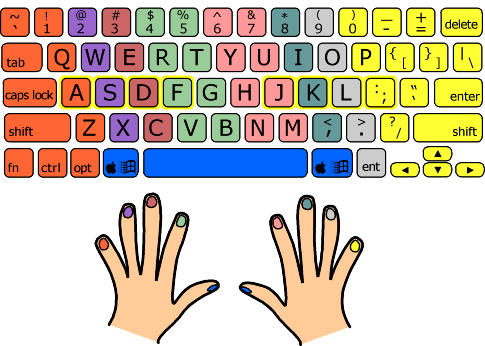
\includegraphics{finger-map.png}

Using this standard finger map, when typing the word \texttt{mummy} on the QWERTY keyboard, you would exclusively use your right index finger to type the entire word, making it significantly slower to type compared to a word like \texttt{there}, which doesn't involve using the same finger to type two consecutive letters.

\begin{textexamples}
\end{textexamples}

The characteristics of how difficult a word is to type extends beyond these two examples, and each characteristic has a different amount of influence on how quickly I type the word. In order to determine the significance of these various characteristics in the difficulty of a word, machine learning can be applied.

\section*{Gathering Data}

In order to create a machine learning algorithm that predicts how fast I can type a certain text based on the text features, we need to collect a large amount of data that includes various texts and the speed at which I type them. Luckily, I've been using TypeRacer for over 5 years now, and over these 5 years I've typed over 8000 texts on my account.

I created a program that automatically scrapes the race data from all my 8000 races and saves them into a file.

% TODO: Why WPM Ratio?

\section*{Analyzing Data}

Thus, to take into consideration the gradual increase in my typing speed overtime, the typing speed of a word should be measured relative to my average speed at the time.

After analyzing the data, I noticed some outliers in the data set. Occasionally, I take a short breather in the middle of a typing race if I'm making too many mistakes, and this is reflected in some of the data as it causes my algorithm to calculate abnormally low speeds for some words. To counter this problem, I decided to take the median of the wpm ratios, as it wouldn't be as affected by outlier data compared to the mean.

\section*{Predicting Typing Speed}

The WPM Ratio of a word depends on various features of the word, such as the length of the word and the amount of capital letters in the word.

For example, if the typing speed of a word was linearly proportional to its length, then our predictive function might look like the following:
\begin{align*}
	\text{WPM Ratio} = w_{\text{word length}} \times (\text{word length}) + \text{Bias}
\end{align*}

This equation resembles the typical linear equation $y = mx + b$, where $w_{\text{word length}}$ represents the slope, or in other words, the amount that the WPM Ratio increases or decreases by when the word length is increased by 1.

However, when we plot the graph of word length against WPM Ratio, we get the following figure:

\begin{figure}[H]
	\caption{Word Length vs. WPM Ratio}
	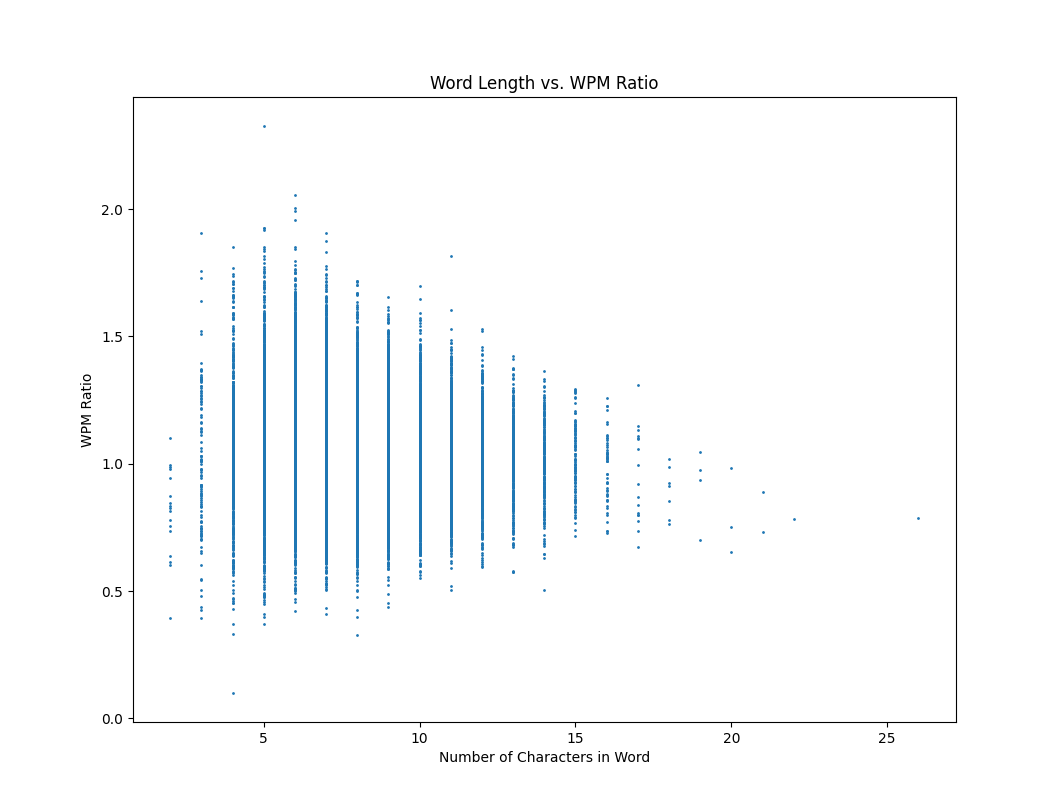
\includegraphics{word-length-vs-wpm.png}
\end{figure}

The graph indicates that longer words typically have lower WPM Ratios, but the range of WPM ratios for shorter words is much larger. If we filter out words that have a WPM ratio lower than 0.5, we can understand why:

% \begin{noindent}
\begin{pycode}
word_stats = [
	word_stat.strip().split('|') for word_stat in """
		"If |0.4905423436151009
		L.A. |0.48295763254168533
		DOS |0.46217555276196115
		"No |0.428899294475664
		'How |0.3993690501499697
		UBS |0.4679134219795311
		GROW |0.4646458701500651
		Six? |0.48037553838088465
	""".strip().splitlines()
]

def get_table():
	table = """
		\\begin{center}
		\\noindent
		\\begin{tabularx}{
			0.5\\linewidth
		}{|X|X|}
		\\hline
		Word (wrapped in ``'') & WPM Ratio
	"""
	for word_stat in word_stats:
		table += f"""
			\\\\\\hline
			``\\code{{{word_stat[0]}}}'' & {"%.3f" % float(word_stat[1])}
		"""
	table += """
		\\\\\\hline
		\\end{tabularx}
		\\end{center}
	"""
	return table
\end{pycode}
% \end{noindent}

\begin{table}
	\caption{Examples of words that are short but have low WPM ratios (i.e. hard to type).}
	\py{get_table()}
\end{table}

Even though these words are short, they contain capital letters and keys that need you to press the Shift key to type (\code{"} and \code{?}). This makes the word substantially slower to type, and isn't accounted for in Equation 1.

Our function must take into account various features of the word that would affect typing speed. Some features, like the number of capital letters, will influence the word's typing speed more compared to other features, like whether the word starts with a vowel or a consonant.

To account for the different influences of different features, we need to assign a different weight to each of them in our equation, which gives us an equation similar to the following:
\begin{align*}
	\text{WPM Ratio} = w_1 \times (\text{Feature 1}) + w_2 \times (\text{Feature 2}) + \dots + \text{Bias}
\end{align*}

For example, if the only two features that influence the difficulty of a are the length of the word and the number of capital letters in the word, then the equation would become:
\begin{align*}
	\text{WPM Ratio} = w_{\text{word length}} \times (\text{word length}) + w_{\text{capital letters}} \times (\text{\# of capital letters}) + \text{Bias}
\end{align*}

In this equation, $w_{\text{word length}}$ isn't necessarily the same as $w_{\text{capital letters}}$. For example, if the magnitude of $w_{\text{word length}}$ is greater than $w_{\text{capital letters}}$, it means that the length of a word has more influence on the WPM ratio compared to the number of capital letters in the word.

Let us define the WPM Ratio as a function that takes in a word $\text{Word}_i$ as input and returns the sum of the feature weights multiplied with the feature values of $\text{Word}_i$. If $w_i$ represents the weight for feature $i$, $x_{f_i}$ represents the feature value for feature $f$ of word $i$, and $b$ represents the bias term, then our WPM ratio equation can be written as:
\begin{align*}
	f(\text{Word}_i) & = w_1{x_1}_i + w_2{x_2}_i + \dots + w_n{x_n}_i + b
	\\
	f(\text{Word}_i) & = \Big(\sum_{f=1}^{n} w_f{x_f}_i\Big) + b
\end{align*}

In this equation, $f$ is our prediction function: given a word, it predicts the WPM ratio of the word based on its features. To create an accurate prediction function, we need to find optimal values of $w_f$ that will give us predicted WPM ratios that are as close as possible to actual WPM ratios from our data. To find optimal values of $w_f$, we need to use a cost function.

\subsection*{The Cost Function}

The cost function will give us a way to measure how accurate our prediction function $f$ is, and more importantly, how we can adjust the weights $w_i$ in our prediction function in order to reduce the cost.

One popular cost function used in machine learning is the MSE (Mean Squared Error). This function defines the cost as the squares of the difference between the actual data ($y_i$) and the predicted data ($f(\text{Word}_i)$):
\begin{align*}
	C(f) & = \frac{1}{N}\big[(y_1 - f(\text{Word}_1))^2 + (y_2 - f(\text{Word}_2))^2 + \dots + (y_n - f(\text{Word}_n))^2]
	\\
	C(f) & = \frac{1}{N} \sum_{i=1}^{n} (y_i - f(\text{Word}_i))^2
\end{align*}

To visualize this cost function, I've plotted the below data for a small set of words that have a clear correlation between word length and WPM Ratio:

% \begin{noindent}
\begin{pycode}
word_data = [
	['month.', 6, 1.8523997581589209],
	['should ', 7, 1.7302841332533008],
	['meaning.', 8, 1.614390135538142],
	['singing. ', 9, 1.5007211799003408],
	['thoughts. ', 10, 1.448833713008257],
	['standpoint ', 11, 1.3051500032628751],
]

def get_table_row(row_index: int):
	return f"""
		\\\\\\hline
		``{word_data[row_index][0]}'' &
		{word_data[row_index][1]} &
		{"%.3f" % word_data[row_index][2]}
	"""
def f3f(number):
	return "%.3f" % number
\end{pycode}
% \end{noindent}

\begin{table}[H]
	\caption{The word length and WPM ratio for a small selection of words.}
	\noindent\begin{tabularx}{\linewidth}{|X|X|X|}
		\hline
		Word        &
		Word Length &
		WPM Ratio

		\py{get_table_row(0)}
		\py{get_table_row(1)}
		\py{get_table_row(2)}
		\py{get_table_row(3)}
		\py{get_table_row(4)}
		\py{get_table_row(5)}

		\\\hline
	\end{tabularx}
\end{table}

A visual example of this cost function would look like:

% TODO
\begin{figure}[H]
	\centering
	\caption{A graph of the values in Figure 4, where the blue lines between the line of best fit and the actual data points represent the cost.}
	\includegraphics{mse-cost.png}
\end{figure}

The goal of our machine learning algorithm is to minimize the cost function: to find a set of weights for our prediction function $f$ such that $C(f)$ is as low as possible. A popular method for minimizing cost is by using gradient descent.

\subsection*{Gradient Descent}

Gradient descent involves using the derivative(s) of a function to find a function's local minimum. In our case, we need to find the local minimum of our cost function, $C$.

Let's consider the case where our prediction function $f$ is linearly correlated with only one weight, the text length. If we let $x_i$ represent the "text length of word $i$", our prediction function would look like the following:
\begin{align*}
	f(\text{Word}_i) = w_1x_i + b
\end{align*}

For this definition of $f$, our cost function would look like the following:
\begin{align*}
	C(w_1, b) & = \frac{1}{N} \sum_{i=1}^{n} (y_i - f(\text{Word}_i))^2
	\\
	C(w_1, b) & = \frac{1}{N} \sum_{i=1}^{n} (y_i - w_1x_i - b)^2
\end{align*}

To visualize this cost function, we can use a 3D graph where the x-axis correlates with various values of $w_1$, the z-axis correlates with various values of $b$, and the y-axis represents the cost (the value of $C(w_1, b)$). Using the values from Table 2 for our values of $x_i$ and $y_i$, a visual representation of our cost function would look like the following graph:
\begin{figure}[H]
	\centering
	\caption{A 3D visualization of our cost function.}
	\includegraphics{cost-function.png}
\end{figure}

The goal of our machine learning algorithm is to minimize this cost function. In other words, our goal is to find the minimum on the graph of $C(w_1, b)$. To find the minimum, we need to use the derivatives of $C(w_1, b)$. In particular, since our cost function has more than one variable, $w_1$ and $b$, we need to use partial derivatives.

\subsection*{Partial Derivatives}

For a function that takes multiple variables, the gradient of the function is a vector where the $i$th value in the vector is the partial derivative of our function with respect to variable $i$. For our cost function, this means that the gradient, $\nabla Q$, is equal to:
\begin{align*}
	\nabla Q = \Big(\frac{dC}{dw_1}, \frac{dC}{db}\Big)
\end{align*}

When calculating each partial derivative, the other input variables for the function are treated as constants. For example, when calculating $\frac{dC}{dw_1}$, the bias term $b$ is treated as a constant:
\begin{align*}
	C(w_1, b)       & = \frac{1}{N} \sum_{i=1}^{n} (y_i - w_1x_i - b)^2
	\\
	\frac{dC}{dw_1} & = \frac{1}{N} \sum_{i=1}^{n} 2(y_i - w_1x_i - b) \times -x_i
	\\
	\frac{dC}{dw_1} & = -\frac{2}{N} \sum_{i=1}^{n} (y_i - w_1x_i - b) \times x_i
\end{align*}

Likewise, when calculating $\frac{dC}{db}$, the weight $w_1$ is treated as a constant:
\begin{align*}
	C(w_1, b)     & = \frac{1}{N} \sum_{i=1}^{n} (y_i - w_1x_i - b)^2
	\\
	\frac{dC}{db} & = \frac{1}{N} \sum_{i=1}^{n} 2(y_i - w_1x_i - b) \times -1
	\\
	\frac{dC}{db} & = -\frac{2}{N} \sum_{i=1}^{n} (y_i - w_1x_i - b)
\end{align*}

Thus, the gradient $\nabla Q$ of our cost function is equal to:
\begin{align*}
	\nabla Q = \Big(
	 &
	-\frac{2}{N} \sum_{i=1}^{n} (y_i - w_1x_i - b) \times x_i,
	\\
	 & -\frac{2}{N} \sum_{i=1}^{n} (y_i - w_1x_i - b)
	\Big)
\end{align*}

% Partial Derivative Example Calculation

% \begin{noindent}
\begin{pycode}
x_values = [data[1] for data in word_data]
y_values = [data[2] for data in word_data]
bias = -1
weight = 0.3
def get_expanded_summation():
	global weight
	global bias
	equation = ""
	for i, x, y in zip(range(len(x_values)), x_values, y_values):
		if i != 0 and i % 2 == 0:
			equation += "\\\\ &"
		equation += f"\\big[\\big({'%.3f' % y} - ({weight})({x}) - ({bias})\\big) \\times ({x})\\big]"
		if i != len(x_values) - 1:
			equation += "+"
	return equation

def get_cost_derivative():
	global weight
	global bias
	summation_sum = 0
	for x, y in zip(x_values, y_values):
		summation_sum += (y - weight * x - bias) * x
	return (-2 / len(x_values)) * summation_sum

cost_derivative = get_cost_derivative()

cost_derivative_str = "%.2f" % get_cost_derivative()
\end{pycode}
% \end{noindent}

Each partial derivative with respect to a variable tells us how the cost function would change if the variable changed. For example, if $w_1 = \py{weight}$, the partial derivative $\frac{dC}{dw_1}$ is equal to:
\begin{align*}
	\frac{dC}{dw_1} & = -\frac{2}{N} \sum_{i=1}^{n} (y_i - (\py{weight})x_i - (\py{bias})) \times x_i
	\\
	\frac{dC}{dw_1} & =
	\begin{aligned}[t]
		-\frac{2}{\py{len(x_values)}}
		\Big( & \py{get_expanded_summation()}\Big)
	\end{aligned}
	\\
	\frac{dC}{dw_1} & = \py{cost_derivative_str}
\end{align*}

Because the value of $\frac{dC}{dw_1}$ is positive, it indicates that increasing $w_1$ and keeping $b$ constant would increase the value of our cost function $C(w_1, b)$. This means that our current value of $w_1$ is greater than the optimal value of $w_1$, and to minimize our cost function, we need we should decrease $w_1$.

% \begin{noindent}
\begin{pycode}
def get_expanded_summation_bias():
	global weight
	global bias
	equation = ""
	for i, x, y in zip(range(len(x_values)), x_values, y_values):
		if i != 0 and i % 2 == 0:
			equation += "\\\\ &"
		equation += f"\\big[\\big({'%.3f' % y} - ({weight})({x}) - ({bias})\\big)\\big]"
		if i != len(x_values) - 1:
			equation += "+"
	return equation

def get_cost_derivative_bias():
	global weight
	global bias
	summation_sum = 0
	for x, y in zip(x_values, y_values):
		summation_sum += (y - weight * x - bias)
	return (-2 / len(x_values)) * summation_sum

cost_derivative_bias = get_cost_derivative_bias()

cost_derivative_bias_str = "%.2f" % get_cost_derivative_bias()
\end{pycode}
% \end{noindent}

This process is repeated for each partial derivative. For example, with our current bias value $b = \py{bias}$, the partial derivative $\frac{dC}{db}$ is equal to:
\begin{align*}
	\frac{dC}{db} & = -\frac{2}{N} \sum_{i=1}^{n} (y_i - (\py{weight})x_i - (\py{bias}))
	\\
	\frac{dC}{db} & =
	\begin{aligned}[t]
		-\frac{2}{\py{len(x_values)}}
		\Big( & \py{get_expanded_summation_bias()}\Big)
	\end{aligned}
	\\
	\frac{dC}{db} & = \py{cost_derivative_bias_str}
\end{align*}

In this case, since $\frac{dC}{db}$ is negative when $b = \py{bias}$, it indicates that increasing $b$ will decrease the cost. This means that our current value of $b$ is below the optimal value of $b$, and that we should increase it to minimize the cost.

After we know for each variable whether we should increase it or decrease it, the hyperparameter that determines how much we increase/decrease each variable by is called the learning rate, $\eta$. To find the new weight, $w_1'$, we add the current weight $w_1$ to the learning rate times the negative gradient. We use the negative gradient so that when our gradient is positive, we decrease the variable to decrease our cost, and when our gradient is negative, we increase the variable to decrease our cost:
{
\setlength{\abovedisplayskip}{0pt}
\setlength{\belowdisplayskip}{0pt}
\begin{center}
	\noindent\begin{tabularx}{0.8\linewidth}{X X}
		\vbox{
			\begin{align*}
				w_1' & = w_1 + (-\frac{dC}{dw_1} \times \eta)
				\\
				w_1' & = w_1 - \frac{dC}{dw_1} \times \eta
				\\
				w_1' & = \py{weight} - (\py{cost_derivative_str}) \times \eta
			\end{align*}
		}
		 &
		\vbox{
			\begin{align*}
				b' & = b + (-\frac{dC}{db} \times \eta)
				\\
				b' & = b - \frac{dC}{db} \times \eta
				\\
				b' & = \py{bias} - (\py{cost_derivative_bias_str}) \times \eta
			\end{align*}
		}
	\end{tabularx}
\end{center}
}

% \begin{noindent}
\begin{pycode}
learning_rate = 0.01
\end{pycode}
% \end{noindent}

{
\setlength{\abovedisplayskip}{0pt}
\setlength{\belowdisplayskip}{0pt}
For example, if we set $\eta$ equal to \py{learning_rate}, then the new values for our weight and bias are:
\begin{center}
	\begin{tabularx}{0.8\linewidth}{X X}
		\vbox{
			\begin{align*}
				w_1' & = \py{weight} - (\py{cost_derivative_str}) \times \py{learning_rate}
				\\
				w_1' & = \py{weight} - (\py{f3f(cost_derivative * learning_rate)})
				\\
				w_1' & = \py{f3f(weight - cost_derivative * learning_rate)}
			\end{align*}
		} &
		\vbox{
			\begin{align*}
				b' & = \py{bias} - (\py{cost_derivative_bias_str}) \times \py{learning_rate}
				\\
				b' & = \py{bias} - (\py{f3f(cost_derivative_bias * learning_rate)})
				\\
				b' & = \py{f3f(bias - cost_derivative_bias * learning_rate)}
			\end{align*}
		}
	\end{tabularx}
\end{center}
}

However, how do we know what value of $\eta$ we should use? In other words, how much should increase or decrease $w_1$ by? If we increase/decrease the weight by too much, we could end up in a position of higher loss than we were before. If we move increase/decrease the weight too slowly, it will take a long time before we find the minimum:

% TODO
\begin{figure}[H]
	\centering
	\caption{Increasing by too much would overshoot the local minimum; increasing by too little would take too long to reach the local minimum.}
	\includegraphics{}
\end{figure}

The optimal choice of $\eta$ will vary for different situations, but there are heuristics that can help. When the learning rate is too high, the cost function will increase infinitely, so whenever it happens in practice you would decrease the learning rate by a % TODO: forgot the word for "power of 10"

I created a Python program to run the above calculations for the values in Table 2 until the difference between $C(w_1, b)$ and $C(w_1', b')$ was less than $10^-9$, indicating that the machine learning model had converged. I set the learning rate $\eta$ to 0.01, and after 8341 iterations, the program outputted the following values for $w_1$ and $b$ (to 9 decimal places):
\begin{align}
	w_1 = -0.105086863 \\
	b = 2.472476099
\end{align}

If we substitute these values for $w_1$ and $b$ into our prediction function $f$ and plot our function on a graph alongside the data from Table 2, we obtain the following graph:
\begin{figure}[H]
	\centering
	\caption{A graph of our prediction function $f$ using the values from equation 1}
	% TODO: plot the function in Excel
	\includegraphics{}
\end{figure}

In my program, I've also tracked the value of the cost function $C(w_1, b)$ after each iteration. Plotting the cost against the iteration number gives us the following graph:
\begin{figure}[H]
	% TODO
	\centering
	\caption{A graph of cost versus iteration number.}
	\includegraphics{}
\end{figure}

However, as indicated by the graph in Table 3, the WPM ratio isn't just correlated with the word length. Thus, we need to apply our machine learning algorithms for a prediction function that takes into account more features in addition to the word length.

\subsection*{Analyzing More Features}
There are many characteristics of a word that can affect its WPM ratio. Below is a list of features that I will be analyzing and using in creating an accurate prediction function for predicting the WPM ratio of a word:

\begin{itemize}
	\item The number of characters in the word.
	\item The number of capital letters in the word.
	\item The amount of times the same finger is used to type consecutive letters in the word. For example, the word "mummy" requires using the right index finger five times in a row on a QWERTY keyboard.
	\item The number of sets of "double letters" in the word. For example, the word "sheep" has 1 set of double letters, and the word "bittersweet" has two sets of double letters.
	\item The number of letters in the home row of the keyboard (on a QWERTY keyboard, this is the row with the letters "asdf").
	\item The number of letters typed with the left hand.
	\item The number of letters typed with the right hand.
	\item The number of numbers in the word.
	\item The number of letters that require pressing the "Shift" key to type.
	\item Whether the word is common (1 if the word is included within the top 1000 most common English words, and 0 otherwise).
\end{itemize}

I've created a program that extracts these features from every word. Table 3 contains three examples of words processed by my program and the value of each of these features for these words:

% \begin{noindent}
\begin{pycode}
word1 = {"word":"profession ","medianWpm":154.134295227525,"isWordCommon":0,"numCapitalLetters":0,"numConsecutiveFingers":1,"numDoubleLetters":1,"numHomeRowLetters":7,"numLeftHandLetters":5,"numNumbers":0,"numRightHandLetters":5,"numShiftedLetters":0,"wordLength":11}

word2 = {"word":"Table, ","medianWpm":136.84411614875188,"isWordCommon":1,"numCapitalLetters":1,"numConsecutiveFingers":0,"numDoubleLetters":0,"numHomeRowLetters":2,"numLeftHandLetters":3,"numNumbers":0,"numRightHandLetters":3,"numShiftedLetters":1,"wordLength":7}

word3 = {"word":"1950s, ","medianWpm":81.3953488372093,"isWordCommon":0,"numCapitalLetters":0,"numConsecutiveFingers":0,"numDoubleLetters":0,"numHomeRowLetters":1,"numLeftHandLetters":4,"numNumbers":4,"numRightHandLetters":2,"numShiftedLetters":4,"wordLength":7}

def get_table_1_row(w):
	return f"""
		\\\\\\hline
		"{w['word']}" &
		{w['wordLength']} &
		{w['numCapitalLetters']} &
		{w['numConsecutiveFingers']} &
		{w['numDoubleLetters']} &
		{w['numHomeRowLetters']}
	"""

def get_table_2_row(w):
	return f"""
		\\\\\\hline
		"{w['word']}" &
		{w['numLeftHandLetters']} &
		{w['numRightHandLetters']} &
		{w['numNumbers']} &
		{w['numShiftedLetters']} &
		{w['isWordCommon']} &
		{"%.2f" % w['medianWpm']}
	"""
\end{pycode}
% \end{noindent}

\begin{table}[H]
	\caption{Three examples of features in words.  The following data might not match with the data expected from a QWERTY layout, and that's because when analyzing my typing data, I based it off the keyboard layout that I use—the Programmer Dvorak layout (please refer to Figure x in the Appendix)}
	\begin{tabularx}{\linewidth}{|
			p{70pt}|
			>{\RaggedRight}X|
			>{\RaggedRight}X|
			>{\RaggedRight}X|
			>{\RaggedRight}X|
			>{\RaggedRight}X|
			>{\RaggedRight}X|
		}
		\hline

		Word                               &
		\# of Characters                   &
		\# of Capitals                     &
		\# of Same-Finger Consecutive Keys &
		\# of Double Letters               &
		\# of Home Row Letters

		\py{get_table_1_row(word1)}
		\py{get_table_1_row(word2)}
		\py{get_table_1_row(word3)}
		\\\hline
	\end{tabularx}

	\begin{tabularx}{\linewidth}{|
			p{70pt}|
			>{\RaggedRight}X|
			>{\RaggedRight}X|
			>{\RaggedRight}X|
			>{\RaggedRight}X|
			>{\RaggedRight}X|
			>{\RaggedRight}X|
			>{\RaggedRight}X|
		}
		\hline

		Word                          &
		\# of Left Hand Letters       &
		\# of Right Hand Letters      &
		\# of Numbers                 &
		\# of Letters Requiring Shift &
		Is word common?               &
		Median WPM

		\py{get_table_2_row(word1)}
		\py{get_table_2_row(word2)}
		\py{get_table_2_row(word3)}
		\\\hline
	\end{tabularx}
\end{table}

To incorporate all these features into our prediction function, we need to include more terms in our equation. If we define $w_f$ to represent the weight of feature $f$ and the value of feature $f$ of word $i$ as ${x_f}_i$, then our new prediction function would look like:
\begin{align*}
	f(\text{Word}_i) & = w_1{x_1}_i + w_2{x_2}_i + \dots + w_{10}{x_{10}}_i + b
	\\
	f(\text{Word}_i) & = \Big(\sum_{f=1}^{10} w_f{x_f}_i\Big) + b
\end{align*}

Our cost function would also change:
\begin{align*}
	C(f)                          & = \frac{1}{10} \sum_{i=1}^{10} (y_i - f(\text{Word}_i))^2
	\\
	C(w_1, w_2, \dots, w_{10}, b) & = \frac{1}{10} \sum_{i=1}^{n} (y_i - w_1{x_1}_i - w_2{x_2}_i - \dots - w_{10}{x_{10}} - b)
\end{align*}

The new gradient $\nabla Q$ for our cost function would now be:
\begin{align*}
	\nabla Q & = \Big(\frac{dC}{dw_1}, \frac{dC}{dw_2}, \dots, \frac{dC}{dw_{10}}, \frac{dC}{db}\Big)
	\\
	\nabla Q & =
	\begin{aligned}[t]
		\Big(
		 & -\frac{2}{10} \sum_{i=1}^{n} (y_i - w_1{x_1}_i - w_2{x_2}_i - \dots - w_{10}{x_{10}}_i - b) \times {x_1}_i,
		\\
		 & -\frac{2}{10} \sum_{i=1}^{n} (y_i - w_1{x_1}_i - w_2{x_2}_i - \dots - w_{10}{x_{10}}_i - b) \times {x_2}_i,
		\\
		 & \vdots
		\\
		 & -\frac{2}{10} \sum_{i=1}^{n} (y_i - w_1{x_1}_i - w_2{x_2}_i - \dots - w_{10}{x_{10}}_i - b) \times {x_{10}}_i,
		\\
		 & -\frac{2}{10} \sum_{i=1}^{n} (y_i - w_1{x_1}_i - w_2{x_2}_i - \dots - w_{10}{x_{10}}_i - b)
		\Big)
	\end{aligned}
\end{align*}

After each iteration, we need to update all 10 weights:
\begin{align*}
	w_1' & = w_1 - \frac{dC}{dw_1} \times \eta,
	\;
	w_2' = w_2 - \frac{dC}{dw_2} \times \eta,
	\;
	\dots,
	\;
	w_{10}' = w_{10} - \frac{dC}{dw_{10}} \times \eta
	\\
	b'   & = b - \frac{dC}{db} \times \eta
\end{align*}

We can simplify the above equations and the implementation of the machine learning algorithm using vectors.

Let us denote $\vec{X_i}$ as a vector whose length is 10, which is equal to the number of features in each word. $\vec{X_i}$ contains all the values of the features of $\text{Word}_i$. Let us denote $\vec{W}$ as a vector also of length 10 containing all the weights for each feature. Using these vector definitions, we can use vectors to represent our prediction function:
\begin{align*}
	f(\text{Word}_i) & = \Big(\sum_{f=1}^{10} w_f{x_f}_i\Big) + b
	\\
	f(\text{Word}_i) & = \vec{X_i} \cdot \vec{W} + b
\end{align*}

To further simplify this equation, we can define $\vec{X}_i$ as a vector of length 11 instead—1 greater than the number of features in each word. In addition to containing all the values of the features of $\text{Word}_i$, we add a constant 1 to the end of $\vec{X}_i$:
\begin{align*}
	\vec{X}_i = ({x_1}_i, {x_2}_i, \dots, {x_{10}}_i, 1)
\end{align*}

This way, if we redefined $\vec{W}$ to be a vector of length 11 which contains all the weights \textit{and} the bias term:
\begin{align*}
	\vec{W} = (w_1, w_2, \dots, w_{10}, b)
\end{align*}

Our prediction function could then be written as:
\begin{align*}
	f(\text{Word}_i) = \vec{X_i} \cdot \vec{W}
\end{align*}

Since this would be equal to:
\begin{align*}
	f(\text{Word}_i) & = w_1{x_i}_1 + w_2{x_i}_2 + \dots + w_{10}{x_i}_{10} + (1)(b)
	\\
	f(\text{Word}_i) & = \Big(\sum_{f=1}^{10} w_f{x_f}_i\Big) + b
\end{align*}

Which is equal to our initial prediction function.

\bigskip

Using vectors, we can also simplify our cost function:
\begin{align*}
	C(f)       & = \frac{1}{10} \sum_{i=1}^{10} (y_i - f(\text{Word}_i))^2
	\\
	C(\vec{W}) & = \frac{1}{10} \sum_{i=1}^{10} (y_i - \vec{W} \cdot \vec{X_i})^2
\end{align*}

And finally, we can simplify our gradient $\nabla Q$:
\begin{align*}
	\nabla Q & = \Big(\frac{dC}{dw_1}, \frac{dC}{dw_2}, \dots, \frac{dC}{dw_{10}}, \frac{dC}{db}\Big)
	\\
	\nabla Q & =
	\begin{aligned}[t]
		\Big(
		 & -\frac{2}{10} \sum_{i=1}^{n} (y_i - \vec{W} \cdot \vec{X_i}) \times {x_i}_1,
		\\
		 & -\frac{2}{10} \sum_{i=1}^{n} (y_i - \vec{W} \cdot \vec{X_i}) \times {x_i}_2,
		\\
		 & \vdots
		\\
		 & -\frac{2}{10} \sum_{i=1}^{n} (y_i - \vec{W} \cdot \vec{X_i}) \times {x_i}_{10},
		\\
		 & -\frac{2}{10} \sum_{i=1}^{n} (y_i - \vec{W} \cdot \vec{X_i})
		\Big)
	\end{aligned}
\end{align*}

With vectors, updating the weights now becomes a simple one-liner:
\begin{align*}
	\vec{W}' = \vec{W} - \eta\nabla Q
\end{align*}

Not only do vectors allow us to represent our equations more succinctly, but they also make implementing them in code much easier.

\section*{Appendix}

\begin{figure}[H]
	\caption{The Programmer Dvorak Keyboard Layout}
	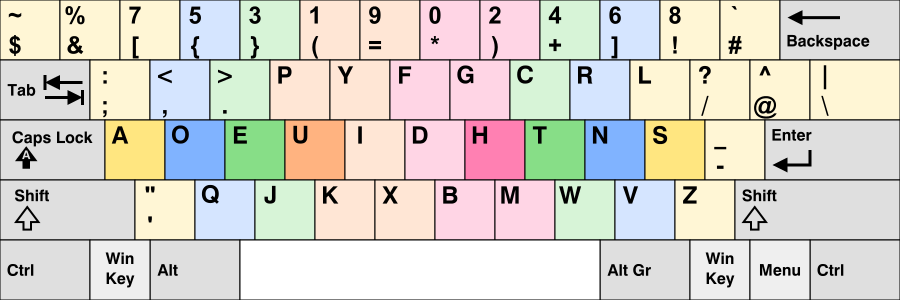
\includegraphics[width=\textwidth]{programmer-dvorak.png}
\end{figure}


\end{document}